% Options for packages loaded elsewhere
\PassOptionsToPackage{unicode}{hyperref}
\PassOptionsToPackage{hyphens}{url}
\documentclass[
]{article}
\usepackage[margin=0.75in]{geometry}
\usepackage{xcolor}
\usepackage{amsmath,amssymb}
\setcounter{secnumdepth}{5}
\usepackage{iftex}
\ifPDFTeX
  \usepackage[T1]{fontenc}
  \usepackage[utf8]{inputenc}
  \usepackage{textcomp} % provide euro and other symbols
\else % if luatex or xetex
  \usepackage{unicode-math} % this also loads fontspec
  \defaultfontfeatures{Scale=MatchLowercase}
  \defaultfontfeatures[\rmfamily]{Ligatures=TeX,Scale=1}
\fi
\usepackage{lmodern}
\ifPDFTeX\else
  % xetex/luatex font selection
\fi
% Use upquote if available, for straight quotes in verbatim environments
\IfFileExists{upquote.sty}{\usepackage{upquote}}{}
\IfFileExists{microtype.sty}{% use microtype if available
  \usepackage[]{microtype}
  \UseMicrotypeSet[protrusion]{basicmath} % disable protrusion for tt fonts
}{}
\makeatletter
\@ifundefined{KOMAClassName}{% if non-KOMA class
  \IfFileExists{parskip.sty}{%
    \usepackage{parskip}
  }{% else
    \setlength{\parindent}{0pt}
    \setlength{\parskip}{6pt plus 2pt minus 1pt}}
}{% if KOMA class
  \KOMAoptions{parskip=half}}
\makeatother
\usepackage{longtable,booktabs,array}
\newcounter{none} % for unnumbered tables
\usepackage{calc} % for calculating minipage widths
% Correct order of tables after \paragraph or \subparagraph
\usepackage{etoolbox}
\makeatletter
\patchcmd\longtable{\par}{\if@noskipsec\mbox{}\fi\par}{}{}
\makeatother
% Allow footnotes in longtable head/foot
\IfFileExists{footnotehyper.sty}{\usepackage{footnotehyper}}{\usepackage{footnote}}
\makesavenoteenv{longtable}
\usepackage{graphicx}
\makeatletter
\newsavebox\pandoc@box
\newcommand*\pandocbounded[1]{#1}%
% Set default figure placement to htbp
\def\fps@figure{htbp}
\makeatother
\setlength{\emergencystretch}{3em} % prevent overfull lines
\providecommand{\tightlist}{%
  \setlength{\itemsep}{0pt}\setlength{\parskip}{0pt}}
% Standard preamble for reslop analysis notes.
% Included via pandoc: --include-in-header=preamble.tex
% Do not edit per-analysis unless you have a specific reason.

% --- Graphics and floats ---
\usepackage{graphicx}
\usepackage{placeins}
\usepackage{float}
\usepackage{needspace}

% Default figure sizing: HEIGHT-based, not width-based.
%
% All figures are produced at figsize=(10,10) — square. But figures
% with colorbars (2D plots, correlation matrices) have extended width
% (e.g., 12x10 effective) due to the colorbar axes. Setting size by
% width makes these figures smaller than 1D plots at the same nominal
% width fraction, because the extra colorbar width eats into the budget.
%
% Setting size by HEIGHT avoids this: a 0.45\linewidth height gives
% consistent visual sizing regardless of colorbars, because the plot
% area height is always 10 inches. Two figures side-by-side at
% height=0.45\linewidth will have matching plot areas even if one has
% a colorbar and the other doesn't.
%
% We unset the default width and set height instead.
\setkeys{Gin}{height=0.45\linewidth,keepaspectratio}

% --- Caption formatting ---
% font=small keeps captions visually distinct from body text.
% Full column width for both figure and table captions.
\usepackage[font=small]{caption}

% --- Tables: prevent page splits ---
% Pandoc generates longtable by default, which splits across pages.
% We strongly discourage this by penalizing breaks inside floats.
% The typesetting agent should also convert longtables to regular
% table floats where the table fits on a single page.
\usepackage{longtable}
\setlength{\LTpre}{0pt}
\setlength{\LTpost}{0pt}

% --- Float placement (relaxed) ---
% LaTeX defaults are too conservative for figure-heavy technical docs.
% These settings allow up to 90% of a page to be floats, preventing
% overfull vbox warnings and figure cutoffs.
\renewcommand{\topfraction}{0.9}
\renewcommand{\bottomfraction}{0.9}
\renewcommand{\textfraction}{0.05}
\renewcommand{\floatpagefraction}{0.6}
\setcounter{topnumber}{3}
\setcounter{bottomnumber}{3}
\setcounter{totalnumber}{6}

% --- Paragraph and page breaking ---
% Prevent widows and orphans (single lines at top/bottom of page).
\widowpenalty=10000
\clubpenalty=10000
% Allow ragged page bottoms rather than stretching vertical glue
% (which creates ugly spacing between paragraphs).
\raggedbottom
\usepackage{bookmark}
\IfFileExists{xurl.sty}{\usepackage{xurl}}{} % add URL line breaks if available
\urlstyle{same}
\hypersetup{
  pdftitle={CMS Open Data H to tau tau Search: Phase 4b 10\% Data Validation},
  pdfauthor={Analysis my\_analysis},
  hidelinks,
  pdfcreator={LaTeX via pandoc}}

\title{CMS Open Data H to tau tau Search: Phase 4b 10\% Data Validation}
\author{Analysis my\_analysis}
\date{2026-06-02}

\begin{document}
\maketitle

{
\setcounter{tocdepth}{3}
\tableofcontents
}
\needspace{4\baselineskip}
\section*{Change Log}\label{change-log}
\addcontentsline{toc}{section}{Change Log}

\textbf{Phase 4b v1}

\begin{itemize}
\tightlist
\item
  Added deterministic 10\% data validation using
  \texttt{(run\ *\ 1000003\ +\ luminosityBlock\ *\ 9176\ +\ event)\ \%\ 10\ ==\ 0}
  on data rows only.
\item
  Added the W high-mT control scale \texttt{0.8433\ ±\ 0.0868}.
\item
  Added fixed-model score-template validation plots for \texttt{vbf},
  \texttt{boosted}, and \texttt{zero\_jet}.
\item
  The remaining 90\% and full-data signal-region distributions remain
  blinded until Phase 4c approval.
\end{itemize}

\needspace{4\baselineskip}
\FloatBarrier
\section{Phase 4b Partial Inference: 10\% Data
Validation}\label{phase-4b-partial-inference-10-data-validation}

\needspace{4\baselineskip}
\subsection{Summary}\label{summary}

Phase 4b validates the Phase 4a expected-primary score-template model on
a deterministic 10\% collision-data subsample. The fitted observable and
category structure are unchanged from Phase 4a:
\texttt{mva\_score\_hist\_gradient\_boosting} in \texttt{vbf},
\texttt{boosted}, and \texttt{zero\_jet} channels with the Phase 4a
score-bin edges. No model retuning, binning optimization, or replacement
method was performed using the 10\% data.

The 10\% mask applies only to data rows and is exactly:
\texttt{(run\ *\ 1000003\ +\ luminosityBlock\ *\ 9176\ +\ event)\ \%\ 10\ ==\ 0}.
MC templates use all selected MC rows but their official Open Data
weights are scaled from \texttt{11.467/fb} to \texttt{1.1467/fb}. The
remaining 90\% and full-data signal-region distributions are not
inspected in this artifact.

\needspace{4\baselineskip}
\subsection{W High-mT Control Scale}\label{w-high-mt-control-scale}

The W+jets high-\texttt{mT} control scale is derived from the masked
10\% data as \texttt{(N\_data\_CR\ -\ nonW\_MC\_CR)\ /\ W\_MC\_CR}. The
control region contains \texttt{400} 10\% data events,
\texttt{W\_MC\ =\ 241.478}, and \texttt{nonW\_MC\ =\ 196.357}. The
applied scale factor is \texttt{0.8433\ ±\ 0.0868} with status
\texttt{valid}. This factor is derived outside the signal region and is
not tuned to improve the score-template agreement.

\needspace{4\baselineskip}
\subsection{Score-Template Validation}\label{score-template-validation}

{\def\LTcaptype{none} % do not increment counter
\vspace{1em}
\begin{table}[htbp]
\centering
\small
\begin{tabular}{@{}
>{\raggedright\arraybackslash}p{(\linewidth - 10\tabcolsep) * \real{0.1304}}
  >{\raggedleft\arraybackslash}p{(\linewidth - 10\tabcolsep) * \real{0.1739}}
  >{\raggedleft\arraybackslash}p{(\linewidth - 10\tabcolsep) * \real{0.1739}}
  >{\raggedleft\arraybackslash}p{(\linewidth - 10\tabcolsep) * \real{0.1739}}
  >{\raggedleft\arraybackslash}p{(\linewidth - 10\tabcolsep) * \real{0.1739}}
  >{\raggedleft\arraybackslash}p{(\linewidth - 10\tabcolsep) * \real{0.1739}}@{}}
\toprule\noalign{}
\begin{minipage}[b]{\linewidth}\raggedright
Category
\end{minipage} & \begin{minipage}[b]{\linewidth}\raggedleft
Data
\end{minipage} & \begin{minipage}[b]{\linewidth}\raggedleft
Background
\end{minipage} & \begin{minipage}[b]{\linewidth}\raggedleft
Data/background
\end{minipage} & \begin{minipage}[b]{\linewidth}\raggedleft
Chi2/ndf
\end{minipage} & \begin{minipage}[b]{\linewidth}\raggedleft
Max abs pull
\end{minipage} \\
\midrule\noalign{}
vbf & 9 & 14.64 & 0.615 & 2.690 & 3.24 \\
boosted & 228 & 205.92 & 1.107 & 0.387 & 0.96 \\
zero\_jet & 883 & 688.35 & 1.283 & 2.121 & 2.01 \\
\end{tabular}
\end{table}
}

Combined over all score-template bins, data/background is \texttt{1.232}
with chi2/ndf \texttt{1.732}. The score-modelling status is
\texttt{flagged} under the predeclared Phase 4b gate.

\needspace{0.4\textheight}
\begin{figure}[htbp]
\centering
\pandocbounded{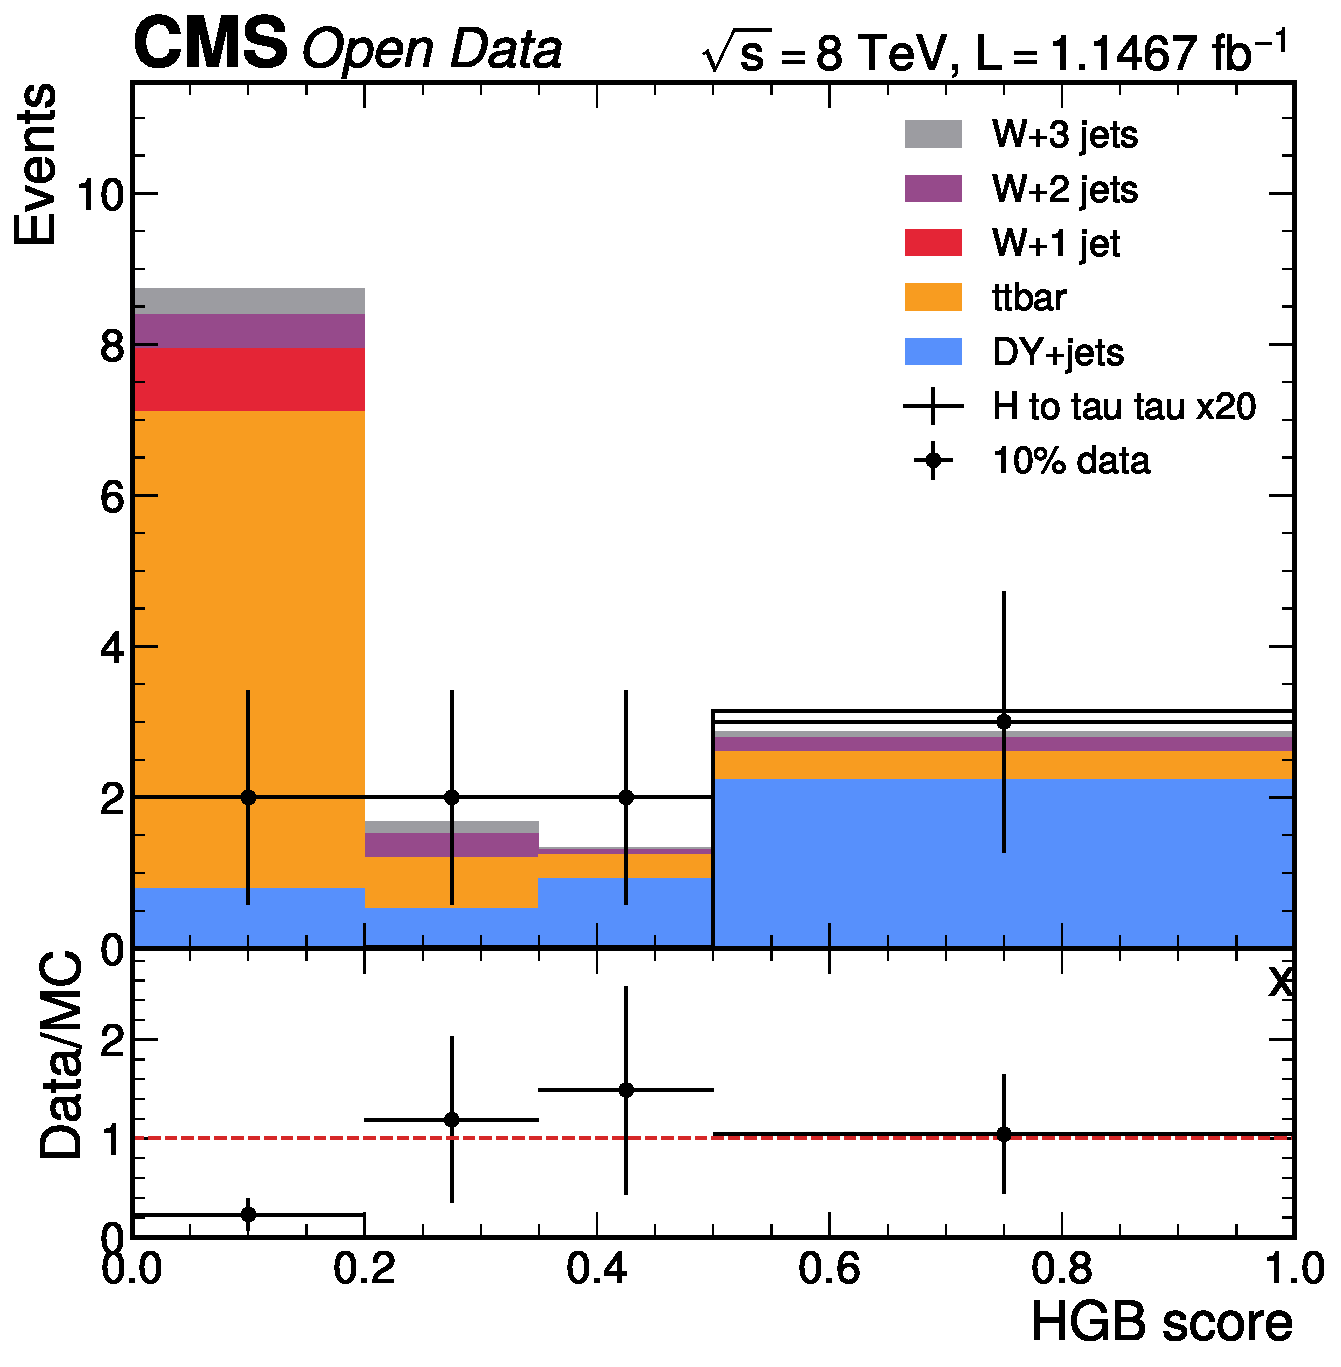
\includegraphics[height=0.35\textheight,width=\linewidth,keepaspectratio,alt={10\% score-template validation in the VBF category. The plot compares the masked 10\% data score distribution to MC normalized to 10\% luminosity with the W high-mT control scale applied. The ratio panel uses the same bins as the Phase 4a pyhf workspace and does not drive any retuning.}]{figures/partial_score_vbf.pdf}}
\caption{10\% score-template validation in the VBF category. The plot
compares the masked 10\% data score distribution to MC normalized to
10\% luminosity with the W high-mT control scale applied. The ratio
panel uses the same bins as the Phase 4a pyhf workspace and does not
drive any retuning.}\label{fig:p4b-score-vbf}
\end{figure}

\needspace{0.4\textheight}
\begin{figure}[htbp]
\centering
\pandocbounded{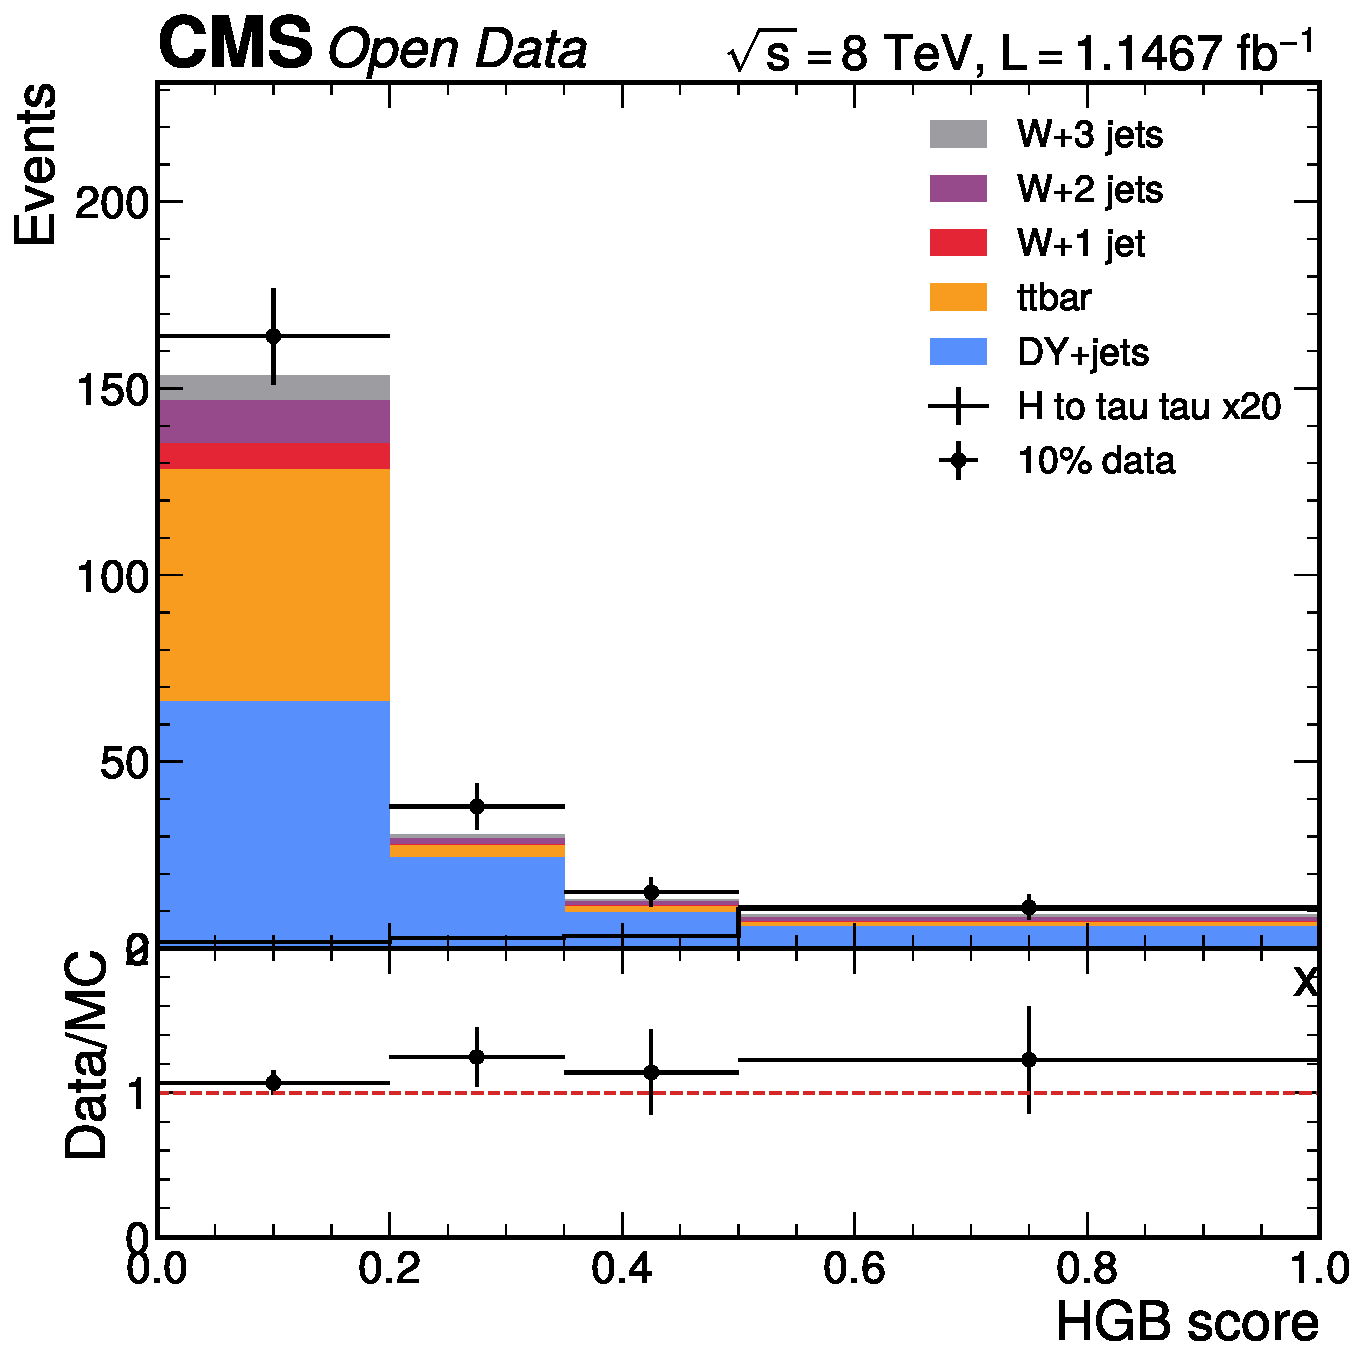
\includegraphics[height=0.35\textheight,width=\linewidth,keepaspectratio,alt={10\% score-template validation in the boosted category. The plot compares the masked 10\% data score distribution to MC normalized to 10\% luminosity with the W high-mT control scale applied. The ratio panel is a validation diagnostic for the fixed Phase 4a model.}]{figures/partial_score_boosted.pdf}}
\caption{10\% score-template validation in the boosted category. The
plot compares the masked 10\% data score distribution to MC normalized
to 10\% luminosity with the W high-mT control scale applied. The ratio
panel is a validation diagnostic for the fixed Phase 4a
model.}\label{fig:p4b-score-boosted}
\end{figure}

\needspace{0.4\textheight}
\begin{figure}[htbp]
\centering
\pandocbounded{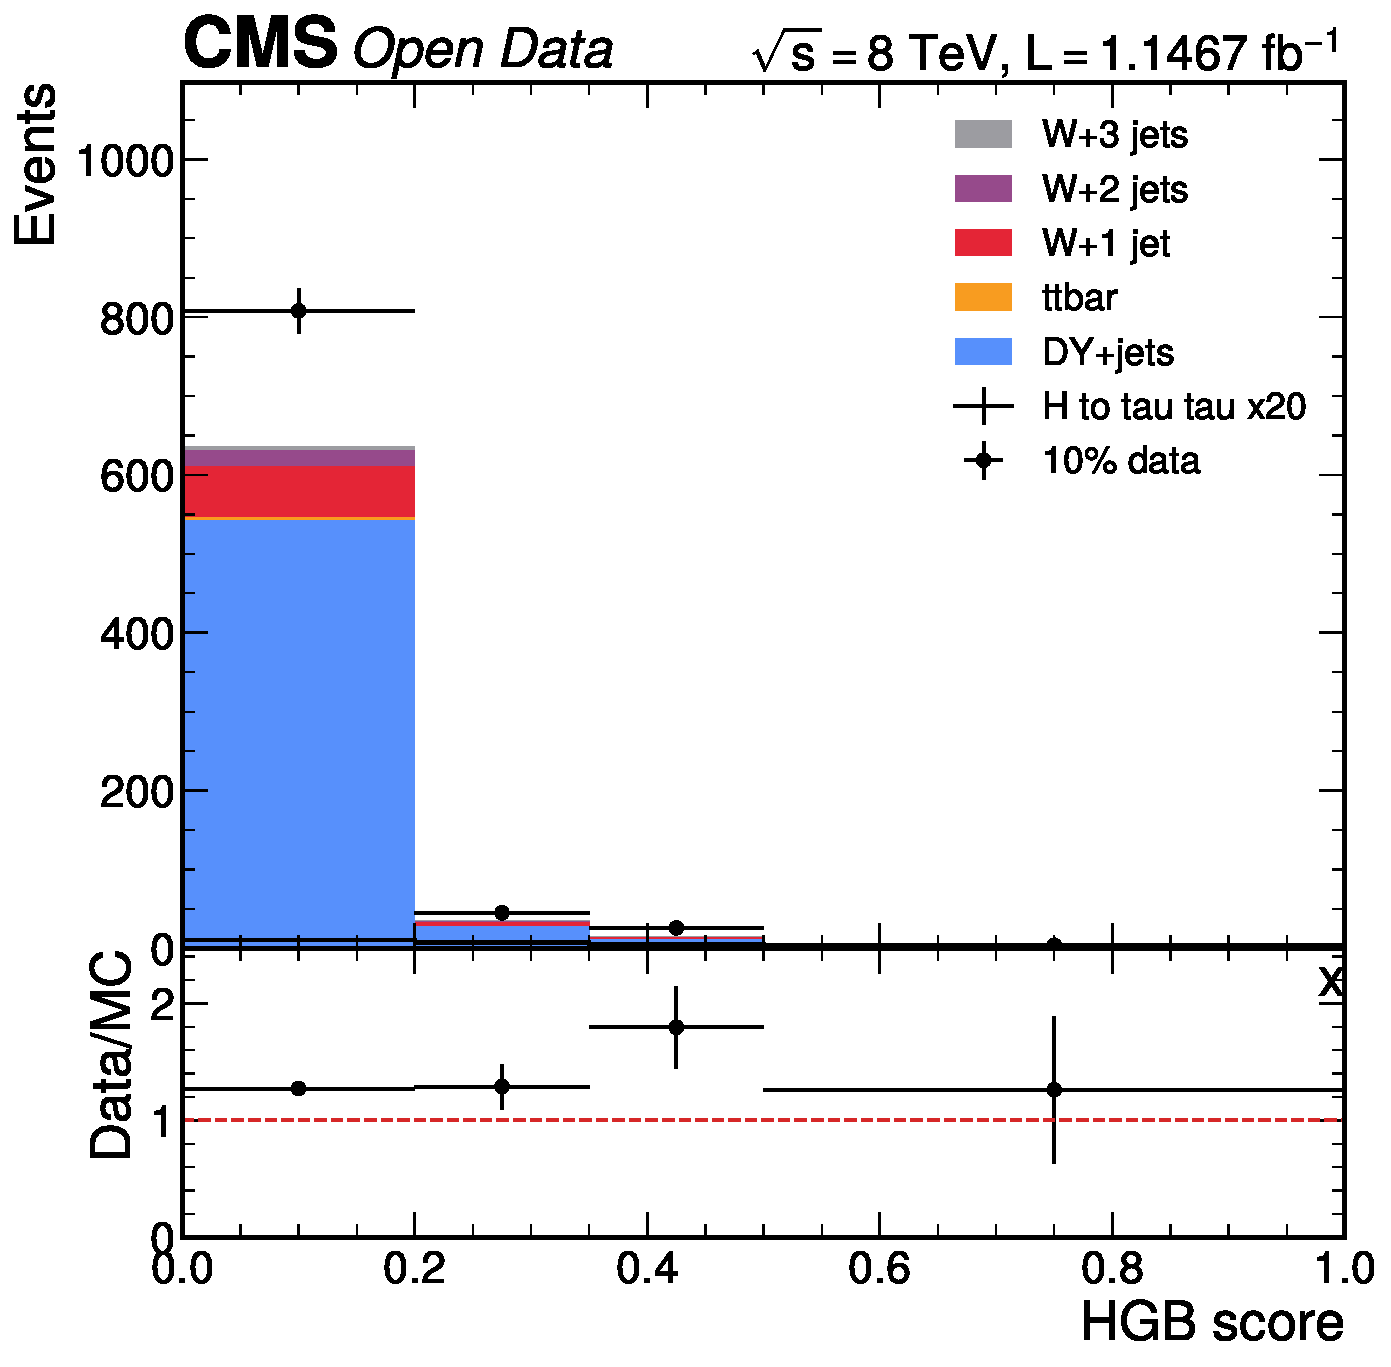
\includegraphics[height=0.35\textheight,width=\linewidth,keepaspectratio,alt={10\% score-template validation in the zero-jet category. The plot compares the masked 10\% data score distribution to MC normalized to 10\% luminosity with the W high-mT control scale applied. This category dominates the event count and therefore the combined ratio.}]{figures/partial_score_zero_jet.pdf}}
\caption{10\% score-template validation in the zero-jet category. The
plot compares the masked 10\% data score distribution to MC normalized
to 10\% luminosity with the W high-mT control scale applied. This
category dominates the event count and therefore the combined
ratio.}\label{fig:p4b-score-zero}
\end{figure}

\needspace{0.4\textheight}
\begin{figure}[htbp]
\centering
\pandocbounded{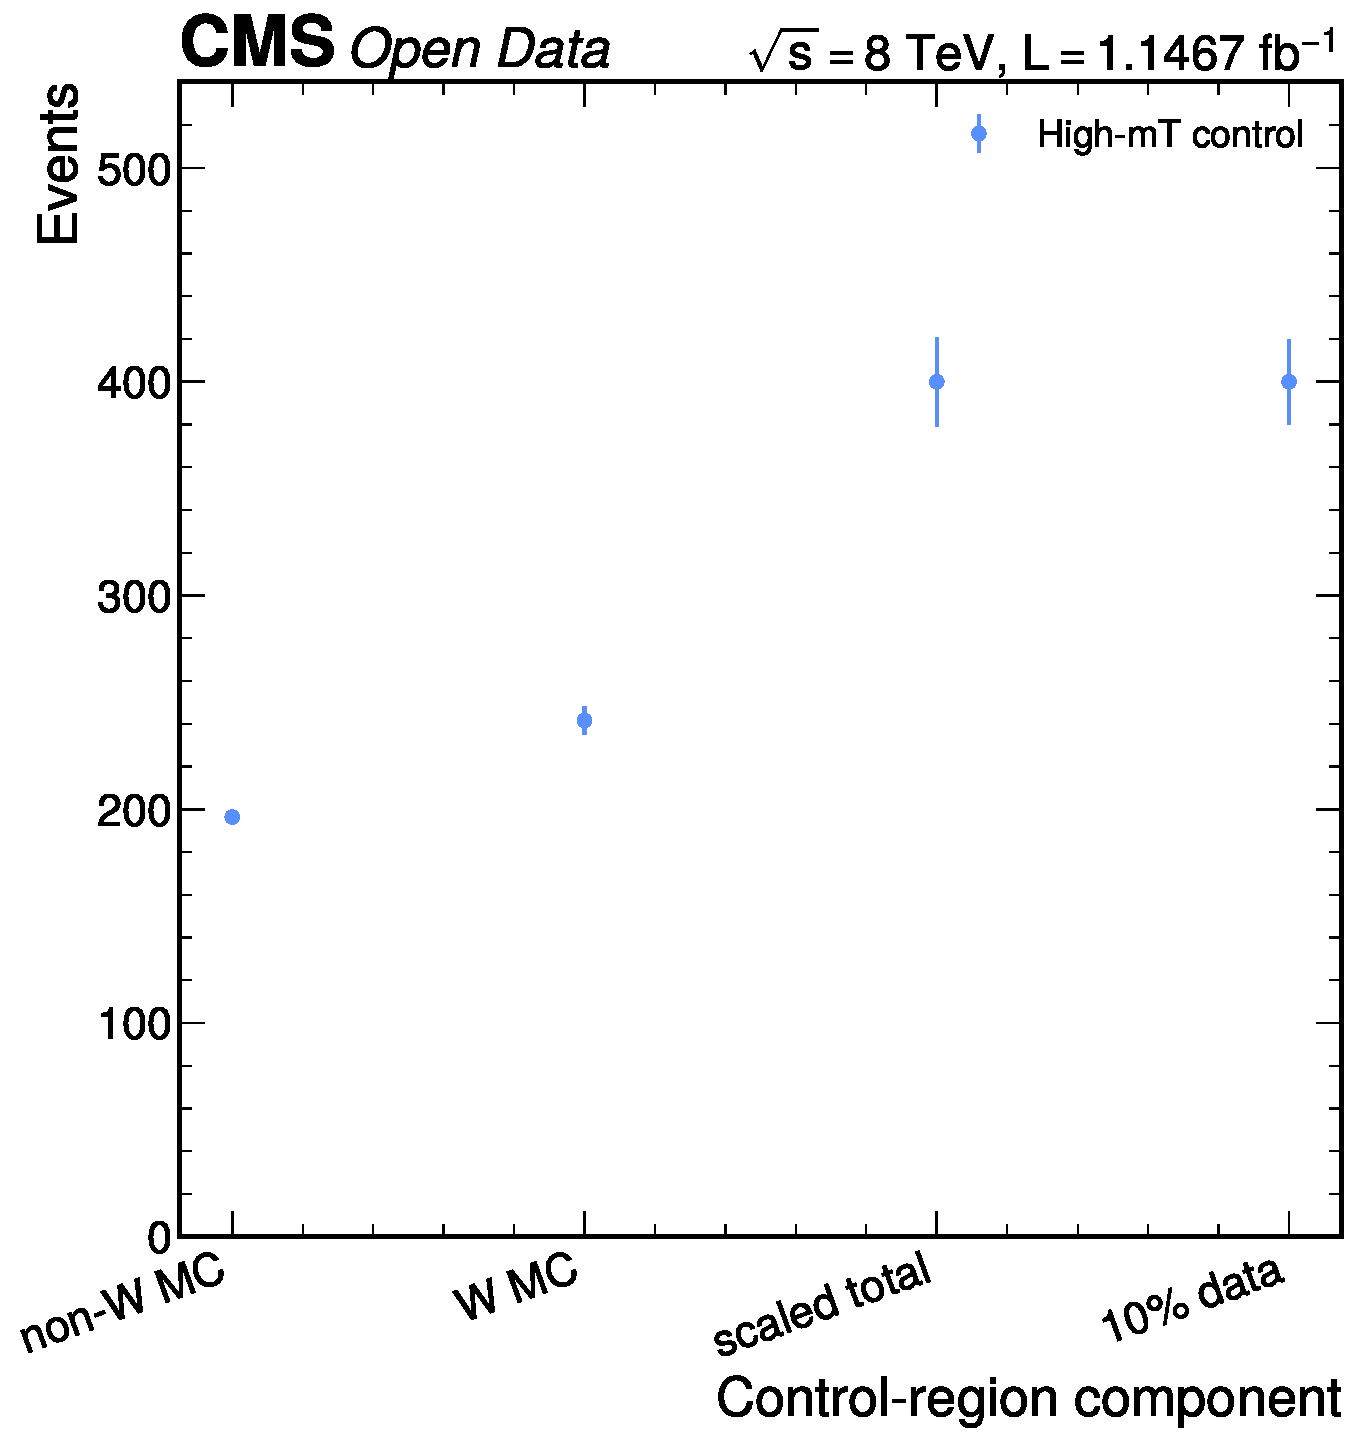
\includegraphics[height=0.35\textheight,width=\linewidth,keepaspectratio,alt={W high-mT control comparison. The figure shows the observed 10\% data control count against the expected W and non-W MC components at 10\% luminosity. The derived scale is propagated to W+jets in the partial workspace as a control region constraint.}]{figures/w_highmt_scale.pdf}}
\caption{W high-mT control comparison. The figure shows the observed
10\% data control count against the expected W and non-W MC components
at 10\% luminosity. The derived scale is propagated to W+jets in the
partial workspace as a control region constraint.}\label{fig:p4b-wcr}
\end{figure}

\needspace{0.4\textheight}
\begin{figure}[htbp]
\centering
\pandocbounded{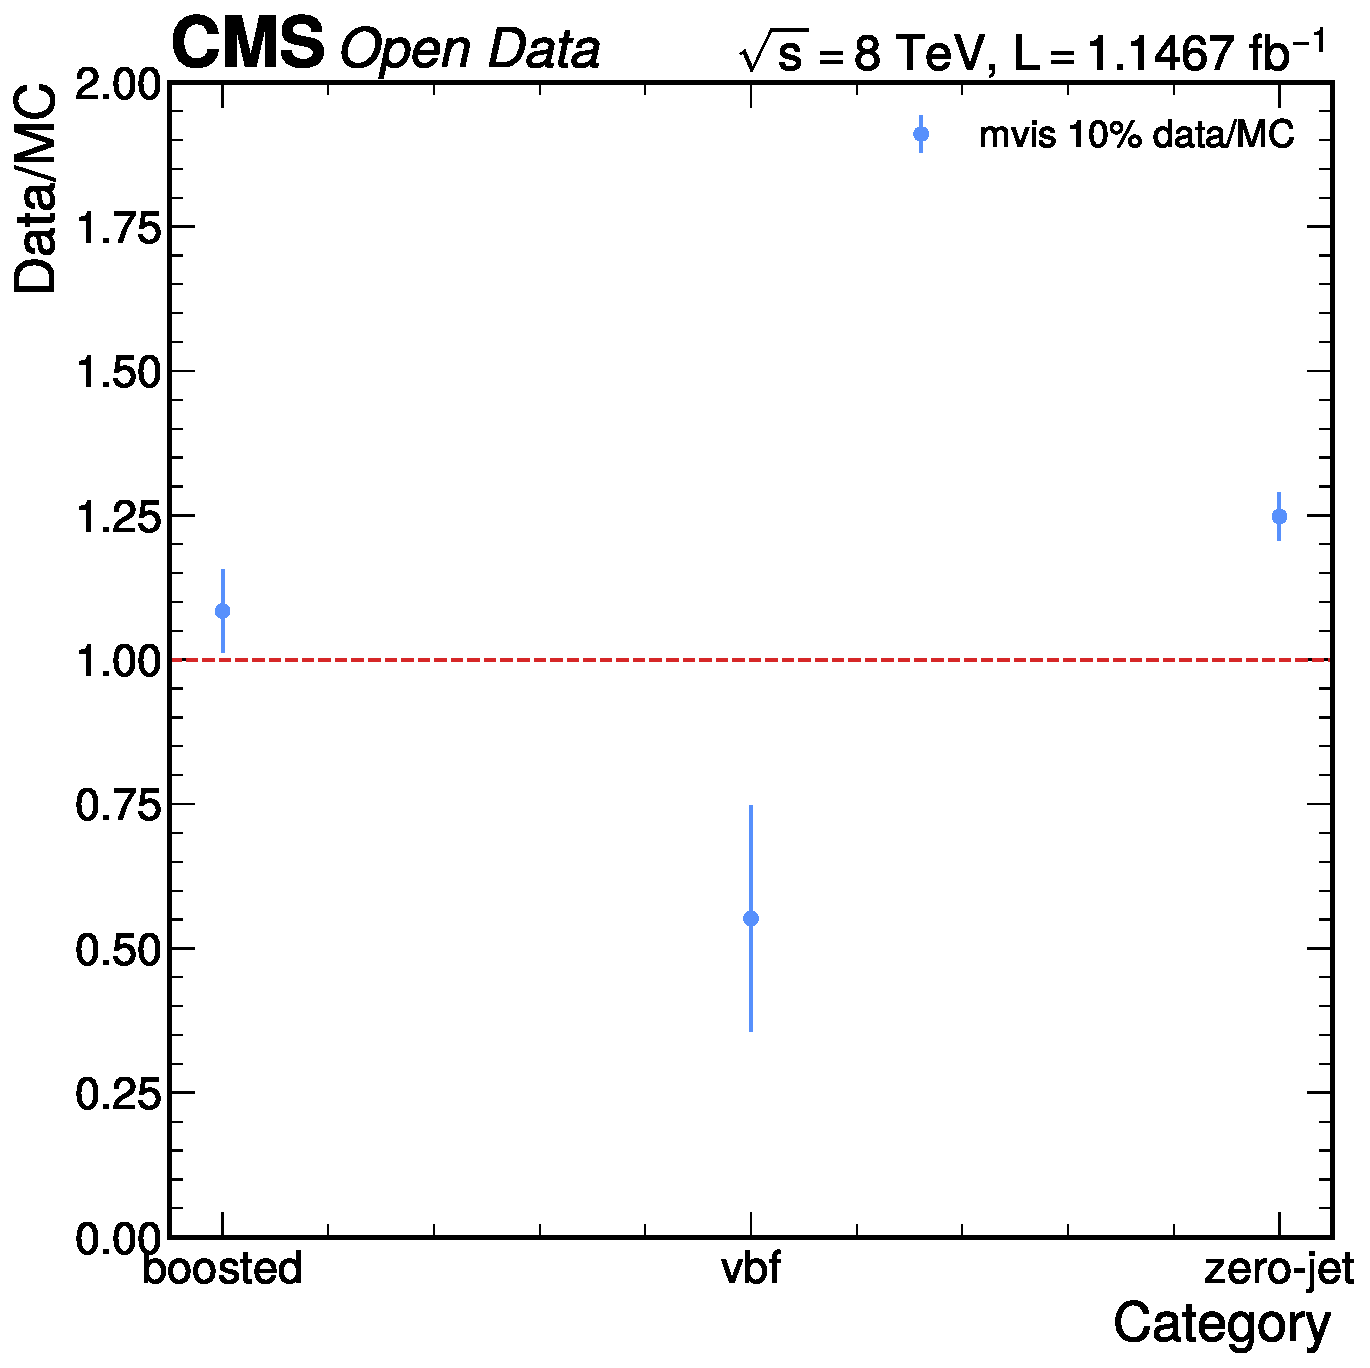
\includegraphics[height=0.35\textheight,width=\linewidth,keepaspectratio,alt={Visible-mass validation summary. The figure provides a mass-shape cross-check using the same masked 10\% data and fixed categories. It is auxiliary to the score-template validation and is not used to choose a new observable.}]{figures/partial_mvis_summary.pdf}}
\caption{Visible-mass validation summary. The figure provides a
mass-shape cross-check using the same masked 10\% data and fixed
categories. It is auxiliary to the score-template validation and is not
used to choose a new observable.}\label{fig:p4b-mvis}
\end{figure}

\needspace{0.4\textheight}
\begin{figure}[htbp]
\centering
\pandocbounded{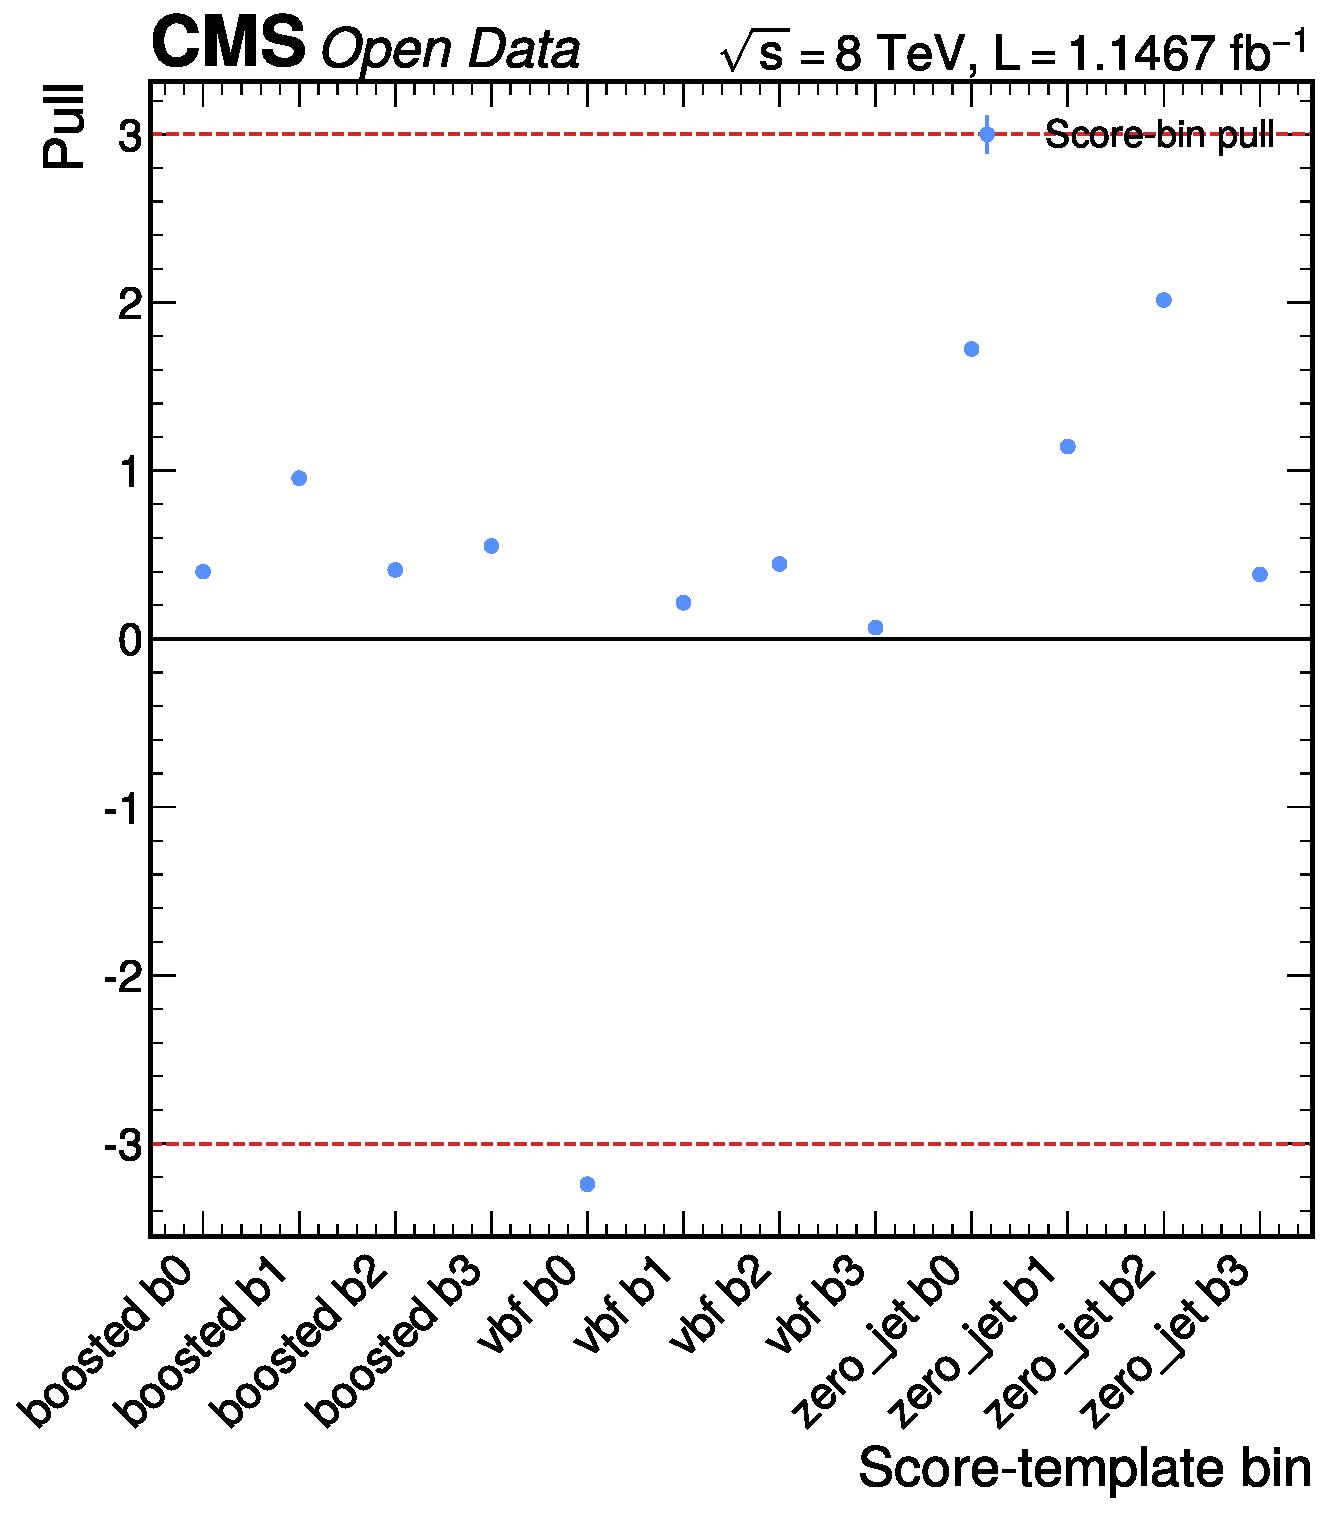
\includegraphics[height=0.35\textheight,width=\linewidth,keepaspectratio,alt={Score-validation pull summary. The figure summarizes per-bin pulls across the three score-template channels using the diagonal validation covariance. It highlights the largest observed 10\% deviations without changing the model.}]{figures/partial_pull_summary.pdf}}
\caption{Score-validation pull summary. The figure summarizes per-bin
pulls across the three score-template channels using the diagonal
validation covariance. It highlights the largest observed 10\%
deviations without changing the model.}\label{fig:p4b-pulls}
\end{figure}

\needspace{4\baselineskip}
\subsection{Partial Diagnostic Fit}\label{partial-diagnostic-fit}

The partial pyhf workspace in \texttt{pyhf\_workspace\_partial.json}
uses the masked 10\% signal-region observations. The diagnostic fit
status is \texttt{evaluated}. If evaluated, its fitted signal strength
is reported only as a 10\%-data validation number and not as a final
result.

\needspace{4\baselineskip}
\subsection{Reproduction}\label{reproduction}

Run:

{\def\LTcaptype{none} % do not increment counter
\vspace{1em}
\begin{table}[htbp]
\centering
\small
\begin{tabular}{@{}
>{\raggedright\arraybackslash}p{(\linewidth - 2\tabcolsep) * \real{0.5000}}
  >{\raggedright\arraybackslash}p{(\linewidth - 2\tabcolsep) * \real{0.5000}}@{}}
\toprule\noalign{}
\begin{minipage}[b]{\linewidth}\raggedright
Command
\end{minipage} & \begin{minipage}[b]{\linewidth}\raggedright
Purpose
\end{minipage} \\
\midrule\noalign{}
\texttt{pixi\ run\ phase4b-results} & Build partial JSON, NPZ,
workspace, and markdown outputs. \\
\texttt{pixi\ run\ phase4b-plots} & Render Phase 4b figures and compile
the minimal 4b note. \\
\texttt{pixi\ run\ phase4b-validate} & Validate blinding metadata,
workspace construction, and figures. \\
\texttt{pixi\ run\ phase4b-all} & Run the full Phase 4b executor
chain. \\
\end{tabular}
\end{table}
}

\needspace{4\baselineskip}
\FloatBarrier
\section{Phase 4a Context}\label{phase-4a-context}

The Phase 4a expected model is the simultaneous pyhf score-template fit
in \texttt{vbf}, \texttt{boosted}, and \texttt{zero\_jet} channels using
\texttt{mva\_score\_hist\_gradient\_boosting} with bin edges
\texttt{{[}0.0,\ 0.2,\ 0.35,\ 0.5,\ 1.0{]}}. Phase 4a reported a median
expected 95\% CLs upper limit of \texttt{4.199} and an expected
discovery diagnostic of \texttt{Z\ =\ 0.526}.

\needspace{4\baselineskip}
\FloatBarrier
\section{Unblinding Checklist}\label{unblinding-checklist}

{\def\LTcaptype{none} % do not increment counter
\vspace{1em}
\begin{table}[htbp]
\centering
\small
\begin{tabular}{@{}
>{\raggedright\arraybackslash}p{(\linewidth - 2\tabcolsep) * \real{0.5000}}
  >{\raggedright\arraybackslash}p{(\linewidth - 2\tabcolsep) * \real{0.5000}}@{}}
\toprule\noalign{}
\begin{minipage}[b]{\linewidth}\raggedright
Gate item
\end{minipage} & \begin{minipage}[b]{\linewidth}\raggedright
Phase 4b status
\end{minipage} \\
\midrule\noalign{}
Background model validated on 10\% data & \texttt{flagged} \\
Systematics retained & luminosity 2.6\%, DY 15\%, tau/open-data 15\%, W
high-mT control \\
Expected result physically sensible & inherited from Phase 4a expected
artifacts \\
Signal injection/closure & inherited from Phase 4a expected artifacts \\
10\% partial unblinding pathologies & see score-template and W high-mT
validation summaries \\
Remaining data blinded & yes \\
\end{tabular}
\end{table}
}
\clearpage

\needspace{4\baselineskip}
\section*{References}\label{references}
\addcontentsline{toc}{section}{References}

\end{document}
